%%%%%%%%%%%%%%%%%%%%%%%%%%%%%%%%%%%%%%%%%%%%%%%%%%%%%%%%%%%%
%% INFORME DE LABORATORIO - UNIVERSIDAD MILITAR NUEVA GRANADA
%% PROGRAMA DE INGENIERÍA MECATRÓNICA
%% CORTE 2: ROBOT MÓVIL INTELIGENTE BASADO EN ESP32
%%%%%%%%%%%%%%%%%%%%%%%%%%%%%%%%%%%%%%%%%%%%%%%%%%%%%%%%%%%%

\documentclass[journal]{IEEEtran}
\IEEEoverridecommandlockouts

%%%%%%%%%%%%%%%%%%%%%%%%%%%%%%
%%%% PAQUETES PRINCIPALES %%%%
%%%%%%%%%%%%%%%%%%%%%%%%%%%%%%
%% Orden: codificación e idioma -> figuras/tablas -> matemáticas ->
%% tikz -> hyperref al final (recomendado).
\usepackage[utf8]{inputenc}
\usepackage[T1]{fontenc}
\usepackage[spanish,es-tabla]{babel}
\usepackage{graphicx}
\usepackage{fancyhdr}
\usepackage{color}
\usepackage{xcolor}
\usepackage{wrapfig}
\usepackage{array}
\usepackage{multirow}
\usepackage{adjustbox}
\usepackage{amsmath}
\usepackage{nccmath}
\usepackage{amsfonts,latexsym}
\usepackage{enumerate}
\usepackage{booktabs}
\usepackage{float}
\usepackage{threeparttable}
\usepackage{array,colortbl}
\usepackage{ifpdf}
\usepackage{rotating}
\usepackage{cite}
%% stfloats es opcional (flotantes a dos columnas en el pie).
\IfFileExists{stfloats.sty}{\usepackage{stfloats}}{}
\usepackage{url}
\usepackage{listings}
\usepackage{makecell}
\usepackage{tikz}
\usetikzlibrary{arrows.meta,positioning,shapes.geometric,fit,calc}
%% hyperref se carga al final para evitar conflictos con el resto.
\usepackage{hyperref}

\setcellgapes{2pt}
\newcolumntype{P}[1]{>{\centering\arraybackslash}p{#1}}
\newcommand{\tabitem}{~~\llap{\textbullet}~~}
\newcommand{\ctt}{\centering\scriptsize\textbf}
\newcommand{\dtt}{\scriptsize\textbf}
\renewcommand\IEEEkeywordsname{Palabras clave}

\graphicspath{{figs/}}

\hypersetup{
    colorlinks=true,
    linkcolor=black,
    citecolor=black,
    urlcolor=blue,
    pdftitle={Robot móvil inteligente basado en ESP32},
    pdfauthor={Kevin Estivem Parra Oñate, Andres Felipe Escovedo Garzon, Camilo Santiago Alvarez Sierra}
}

\hyphenation{mi-cro-con-tro-la-dor co-mu-ni-ca-ción sen-so-res}

%%%%%%%%%%%%%%%%%%%%%%%%%%%%%%%%%%%%%%%%%%%%%%%%%%%%%%%%%%
%%%%%%%%%%% ENCABEZADO TIPO UMNG %%%%%%%%%%%%%%%%%%%%%%%%%
%%%%%%%%%%%%%%%%%%%%%%%%%%%%%%%%%%%%%%%%%%%%%%%%%%%%%%%%%%

\newcommand{\MYhead}{\smash{\scriptsize
\hfil\parbox[t][\height][t]{\textwidth}{\centering
\begin{picture}(0,0)
\put(-0,-17){\IfFileExists{LogoUMNG}{\includegraphics[width=27mm]{LogoUMNG}}{}}
\end{picture}
\hspace{5.4cm}
INFORME DE PROYECTO DE LABORATORIO
\hspace{3.5cm} Versión 1.0\\
\hspace{5.2cm}
PROGRAMA DE INGENIERÍA MECATRÓNICA
\hspace{3.0cm} Periodo 2026-2\\
\underline{\hspace{\textwidth}}}\hfil\hbox{}}}

\makeatletter
\def\ps@headings{%
\def\@oddhead{\MYhead}%
\def\@evenhead{\MYhead}}
\def\ps@IEEEtitlepagestyle{%
\def\@oddhead{\MYhead}%
\def\@evenhead{\MYhead}}
\makeatother

\pagestyle{headings}
\addtolength{\footskip}{0\baselineskip}
\addtolength{\textheight}{-1\baselineskip}

%%%%%%%%%%%%%%%%%%%%%%%%%%%%%%%%%%%%%%%%%%%%%%%%%%%%%%%%%%
%%%% AJUSTE DE COLOCACIÓN DE FIGURAS Y TABLAS %%%%%%%%%%%%%
%%%%%%%%%%%%%%%%%%%%%%%%%%%%%%%%%%%%%%%%%%%%%%%%%%%%%%%%%%
\setcounter{topnumber}{3}
\setcounter{bottomnumber}{2}
\setcounter{totalnumber}{4}
\setcounter{dbltopnumber}{3}
\renewcommand{\topfraction}{0.9}
\renewcommand{\bottomfraction}{0.7}
\renewcommand{\textfraction}{0.08}
\renewcommand{\floatpagefraction}{0.7}
\renewcommand{\dbltopfraction}{0.9}
\renewcommand{\dblfloatpagefraction}{0.7}

%%%%%%%%%%%%%%%%%%%%%%%%%%%%%%%%%%%%%%%%%%%%%%%%%%%%%%%%%%
%%%%%%%%%%%%%%%%%%%% INICIO DOCUMENTO %%%%%%%%%%%%%%%%%%%%
%%%%%%%%%%%%%%%%%%%%%%%%%%%%%%%%%%%%%%%%%%%%%%%%%%%%%%%%%%

\begin{document}

%%%%%%%%%%%%%%%%%%%%%%%%%%%%
%%%%%%%% TÍTULO %%%%%%%%%%%%
%%%%%%%%%%%%%%%%%%%%%%%%%%%%

\title{Robot móvil inteligente basado en ESP32: arquitectura, diseño de subsistemas y desarrollo de control inalámbrico para navegación manual y autónoma}

%%%%%%%%%%%%%%%%%%%%%%%%%%%%
%%%%%%%% AUTORES %%%%%%%%%%%
%%%%%%%%%%%%%%%%%%%%%%%%%%%%

\author{
Kevin~Estivem~Parra~Oñate,
Andres~Felipe~Escovedo~Garzon,
y~Camilo~Santiago~Alvarez~Sierra\\
\textit{Universidad Militar Nueva Granada, Programa de Ingeniería Mecatrónica}\\
Asignatura: Laboratorio de Micros\\
Profesor: Diego Alejandro Barragán Vargas\\
\thanks{Informe correspondiente a la segunda entrega del proyecto de robot móvil inteligente, periodo académico 2026-2. El documento separa los avances de software de las partes de diseño e integración física que todavía deben validarse.}
}

\maketitle

%%%%%%%%%%%%%%%%%%%%%%%%%%%%
%%%%%%%% RESUMEN %%%%%%%%%%%
%%%%%%%%%%%%%%%%%%%%%%%%%%%%

\begin{abstract}
Este informe presenta la arquitectura y el estado de desarrollo de un robot móvil inteligente basado en el microcontrolador ESP32. El proyecto usa una plataforma diferencial de dos ruedas motrices y una rueda de apoyo. El robot está pensado para recibir órdenes manuales y de voz, medir su orientación con una brújula digital, reconocer seis colores, detectar obstáculos y enviar telemetría a una aplicación web hecha con HTML y JavaScript. La comunicación entre la aplicación y el robot se plantea por Wi-Fi y WebSocket, mientras que un asistente llamado JARVIS usa reglas de software para explicar el sistema y responder preguntas sobre las variables disponibles. Se describen los requisitos funcionales y no funcionales, la arquitectura por módulos, los componentes elegidos, la asignación preliminar de pines, el protocolo de comunicación y la máquina de estados global. También se documentan las pruebas de software reportadas y lo que queda pendiente de integración. El diseño CAD está en una etapa inicial, el esquema eléctrico definitivo está pendiente y la comunicación Wi-Fi del firmware todavía no se ha probado con el microcontrolador físico. Por eso, los resultados de software se presentan aparte de las pruebas físicas que faltan por hacer.
\end{abstract}

%%%%%%%%%%%%%%%%%%%%%%%%%%%%
%%%%%%% PALABRAS CLAVE %%%%%%
%%%%%%%%%%%%%%%%%%%%%%%%%%%%

\begin{IEEEkeywords}
ESP32, robot móvil, navegación diferencial, WebSocket, Wi-Fi, brújula digital, detección de colores, evasión de obstáculos, máquina de estados, aplicación web.
\end{IEEEkeywords}

%%%%%%%%%%%%%%%%%%%%%%%%%%%%%%%%%%%%%%%%%%%%%%%%%%%%%%%%%%
%%%%%%%%%%%%%%%%%%%% INTRODUCCIÓN %%%%%%%%%%%%%%%%%%%%%%%%
%%%%%%%%%%%%%%%%%%%%%%%%%%%%%%%%%%%%%%%%%%%%%%%%%%%%%%%%%%

\section{Introducción}

Los robots móviles combinan partes mecánicas, electrónicas y de software para moverse e interactuar con su entorno. Para construirlos hay que coordinar la lectura de los sensores, el procesamiento de los datos, el control de los motores y la comunicación con un operador. En un robot autónomo, además, hay que interpretar lo que ocurre alrededor y decidir cómo moverse.

El ESP32 es el corazón del proyecto. Sobre este microcontrolador se planea una arquitectura por módulos que permita manejar los motores, leer los sensores, controlar los modos de trabajo y enviar datos a una aplicación inalámbrica. Separar el sistema en módulos independientes facilita armarlo por partes y encontrar fallos durante las pruebas.

El sistema se plantea con tracción diferencial: dos ruedas motrices y una rueda de apoyo. La orientación se obtiene con un módulo de brújula digital GY-271, basado en el magnetómetro QMC5883L. El color se detecta con un sensor TCS34725 y los obstáculos con un sensor ultrasónico HC-SR04. Para mover los motores se eligió un controlador TB6612FNG.

La aplicación de supervisión ya está hecha a nivel de software, pero todavía no se ha probado con el ESP32 físico. La comunicación prevista usa Wi-Fi y WebSocket, con mensajes ordenados que permiten pedir cambios de modo, enviar órdenes de movimiento y recibir telemetría. El asistente JARVIS también se hizo con reglas de software. Su conexión con datos físicos reales depende de que la comunicación y los sensores funcionen.

Este documento corresponde al Corte 2 y presenta los requisitos, la arquitectura, las decisiones de diseño y las evidencias de software disponibles. El diseño mecánico está en una etapa inicial y el esquema eléctrico definitivo está pendiente. Por eso no se presentan como resultados experimentales las funciones que aún no se han probado en el prototipo físico.

\section{Objetivos}

\subsection{Objetivo general}

Desarrollar la arquitectura de un robot móvil inteligente basado en ESP32, integrando el diseño mecánico y electrónico con un firmware por módulos y una aplicación inalámbrica para el control manual, la supervisión y la futura navegación autónoma.

\subsection{Objetivos específicos}

\begin{enumerate}[1.]
    \item Identificar los requisitos funcionales y no funcionales del robot y definir una arquitectura por módulos que facilite unir sensores, actuadores, firmware y aplicación de supervisión.

    \item Elegir los componentes electrónicos y definir una asignación preliminar de pines para el ESP32, los motores, los sensores y los elementos de seguridad.

    \item Desarrollar una estructura de firmware por módulos y una máquina de estados que separe los modos manual, autónomo, seguro y de error.

    \item Implementar una aplicación de control y supervisión que use mensajes ordenados por WebSocket para pedir acciones y mostrar telemetría.

    \item Incorporar un asistente JARVIS basado en reglas de software para responder preguntas sobre el funcionamiento del robot y la información disponible.

    \item Definir una metodología de pruebas que permita verificar poco a poco el protocolo, los sensores, el control de motores, la orientación y la navegación, separando los resultados de software de las pruebas físicas que faltan.
\end{enumerate}

%%%%%%%%%%%%%%%%%%%%%%%%%%%%%%%%%%%%%%%%%%%%%%%%%%%%%%%%%%
%%%%%%%%%%%%%%%%%%%% COMPETENCIAS %%%%%%%%%%%%%%%%%%%%%%%%
%%%%%%%%%%%%%%%%%%%%%%%%%%%%%%%%%%%%%%%%%%%%%%%%%%%%%%%%%%

\section{Competencias a desarrollar}

\begin{itemize}
    \item \textbf{Competencia 1.} Diseñar sistemas mecatrónicos que integren partes mecánicas, electrónicas y de software.

    \item \textbf{Competencia 2.} Implementar firmware por módulos para sistemas embebidos, con lectura de sensores, control de actuadores y manejo de estados.

    \item \textbf{Competencia 3.} Desarrollar interfaces de comunicación inalámbrica para supervisar variables y enviar comandos a un sistema embebido.

    \item \textbf{Competencia 4.} Aplicar métodos de verificación y trazabilidad para comprobar los requisitos con pruebas repetibles.

    \item \textbf{Competencia 5.} Analizar las limitaciones de un prototipo y distinguir entre resultados simulados, pruebas de software y mediciones experimentales.
\end{itemize}

%%%%%%%%%%%%%%%%%%%%%%%%%%%%%%%%%%%%%%%%%%%%%%%%%%%%%%%%%%
%%%%%%%%%%%%%%%%%%%% REQUISITOS %%%%%%%%%%%%%%%%%%%%%%%%%%
%%%%%%%%%%%%%%%%%%%%%%%%%%%%%%%%%%%%%%%%%%%%%%%%%%%%%%%%%%

\section{Requisitos del sistema}

Los requisitos se dividen en funcionales y no funcionales. La Tabla~\ref{tab:requisitos} resume las funciones principales y su estado. Cuando dice ``pendiente'' significa que la función necesita más trabajo, integración o validación; no quiere decir que ya se haya probado con éxito en el robot físico.

\begin{table*}[t]
\centering
\caption{Requisitos funcionales y estado de desarrollo}
\label{tab:requisitos}
\scriptsize
\begin{tabular}{p{0.58\textwidth} p{0.32\textwidth}}
\toprule
\textbf{Requisito} & \textbf{Estado} \\
\midrule
Control manual del movimiento del robot desde la aplicación. & Aplicación desarrollada; falta probarla con el ESP32. \\
Interpretar comandos de voz o texto y convertirlos en órdenes de control. & Procesamiento de comandos hecho en software; falta la validación completa. \\
Manejar los modos manual y autónomo con una máquina de estados, sin que funcionen a la vez. & Arquitectura de firmware definida; falta la integración física. \\
Obtener y mostrar la orientación del robot en grados con una brújula digital. & Módulo de sensor previsto; faltan calibración y validación física. \\
Reconocer los colores negro, blanco, rojo, amarillo, verde y azul. & Clasificación evaluada en software; falta la calibración física. \\
Detectar obstáculos y hacer una maniobra de evasión para seguir la trayectoria. & Conversión de distancia lista en software; falta validar la maniobra autónoma. \\
Comunicación inalámbrica con un protocolo con versión y un tiempo de caducidad para los comandos. & Protocolo y pruebas de software listos; falta el Wi-Fi en el firmware. \\
Mostrar controles y telemetría en una aplicación web. & Aplicación hecha; falta conectarla con el ESP32 físico. \\
Incorporar un asistente JARVIS que explique el proyecto y responda sobre la información disponible. & Asistente por reglas hecho en software; falta conectarlo a las variables físicas. \\
\bottomrule
\end{tabular}
\end{table*}

\subsection{Requisitos no funcionales}

Se consideran los siguientes requisitos de calidad y seguridad:

\begin{itemize}
    \item \textbf{Seguridad:} ante una parada de emergencia, una pérdida de comunicación o un error, el sistema debe quedar en un estado seguro que impida mover los motores sin querer.

    \item \textbf{Ejecución sin bloqueos:} las tareas de sensores, comunicación y control deben estar organizadas para no quedarse esperando y poder atender siempre los eventos de seguridad.

    \item \textbf{Modularidad:} cada sensor, actuador, protocolo y estrategia de control debe tener una interfaz definida.

    \item \textbf{Trazabilidad:} cada requisito debe estar relacionado con uno o más módulos y pruebas.

    \item \textbf{Robustez de la comunicación:} los mensajes deben validarse con un campo de versión y un tipo de comando reconocido.

    \item \textbf{Protección de credenciales:} las contraseñas y demás datos de la red no deben publicarse en el repositorio.

    \item \textbf{Control del presupuesto:} al elegir los componentes hay que tener en cuenta el costo total y su disponibilidad.
\end{itemize}

%%%%%%%%%%%%%%%%%%%%%%%%%%%%%%%%%%%%%%%%%%%%%%%%%%%%%%%%%%
%%%%%%%%%%%%%%%%%%%% MARCO TEÓRICO %%%%%%%%%%%%%%%%%%%%%%%
%%%%%%%%%%%%%%%%%%%%%%%%%%%%%%%%%%%%%%%%%%%%%%%%%%%%%%%%%%

\section{Marco teórico}

\subsection{Robot móvil de tracción diferencial}

Un robot diferencial tiene dos ruedas motrices independientes para avanzar y girar. La velocidad de cada rueda define la velocidad del robot y su giro. En un modelo ideal, estas relaciones se escriben como:

\begin{equation}
v = \frac{r}{2}(\omega_R+\omega_L)
\label{eq:velocidad_lineal}
\end{equation}

\begin{equation}
\dot{\theta} = \frac{r}{b}(\omega_R-\omega_L)
\label{eq:velocidad_angular}
\end{equation}

donde $v$ es la velocidad del robot, $\dot{\theta}$ es su velocidad de giro, $r$ es el radio de las ruedas, $\omega_R$ y $\omega_L$ son las velocidades angulares de las ruedas derecha e izquierda, y $b$ es la distancia entre los centros de las ruedas motrices.

Para el proyecto se eligieron ruedas de $6{,}5~\mathrm{cm}$ de diámetro, así que el radio nominal es:

\begin{equation}
r = \frac{6{,}5}{2} = 3{,}25~\mathrm{cm}
\label{eq:radio_rueda}
\end{equation}

La distancia entre las ruedas todavía debe definirse a partir del diseño CAD final. Por eso no se calcula una velocidad de giro final del robot en esta etapa.

\subsection{Brújula digital y orientación}

El módulo GY-271 usa un magnetómetro QMC5883L que mide el campo magnético en tres ejes. La orientación horizontal se puede estimar a partir de esas mediciones después de calibrar el sensor.

En el caso sencillo de un sensor horizontal, el ángulo magnético se obtiene con:

\begin{equation}
\theta_m = \operatorname{atan2}(B_y,B_x)
\label{eq:rumbo}
\end{equation}

donde $B_x$ y $B_y$ son las componentes del campo magnético en los ejes horizontales del sensor. El resultado se pasa a grados y se ajusta al intervalo que use la aplicación.

Esta fórmula es un cálculo básico. En un montaje real hay que corregir las mediciones por desajustes, escalas y perturbaciones del campo causadas por motores, cables con corriente y piezas metálicas. La calibración del módulo y su posición en el chasis quedan pendientes de validación.

\subsection{Error angular}

Para apuntar el robot hacia una dirección deseada hay que calcular la diferencia entre dos ángulos, teniendo en cuenta que son periódicos. Una resta directa puede dar un valor más grande de lo necesario cuando se cruza entre $0^\circ$ y $360^\circ$.

El error angular se define como:

\begin{equation}
e_\theta =
\left((\theta_d-\theta_a+540^\circ)
\bmod 360^\circ\right)-180^\circ
\label{eq:error_angular}
\end{equation}

donde $\theta_d$ es el ángulo deseado y $\theta_a$ es el ángulo actual. Así el error queda en el intervalo $[-180^\circ,180^\circ)$ y se elige el giro más corto. La respuesta de los motores ante este error necesita una estrategia de control y pruebas físicas que aún faltan.

\subsection{Detección de color}

El sensor TCS34725 mide los canales de rojo, verde, azul y un canal de intensidad sin filtro. Con esas lecturas se puede representar el color observado, pero la clasificación depende de la luz, la distancia, la superficie y la calibración.

De forma básica, las lecturas de los canales se normalizan con la intensidad total:

\begin{equation}
\medmath{
R_n=\frac{R}{R+G+B},\quad
G_n=\frac{G}{R+G+B},\quad
B_n=\frac{B}{R+G+B}}
\label{eq:normalizacion_color}
\end{equation}

donde $R$, $G$ y $B$ son las lecturas de cada canal. Si la suma es cero o muy pequeña, la clasificación se considera inválida. Los umbrales para identificar negro, blanco, rojo, amarillo, verde y azul deben obtenerse midiendo el sensor real con la iluminación controlada.

\subsection{Detección ultrasónica de obstáculos}

El sensor HC-SR04 estima la distancia a un objeto a partir del tiempo que tarda un pulso de sonido en ir y volver. La distancia aproximada se calcula con:

\begin{equation}
d=\frac{c\,t}{2}
\label{eq:distancia_ultrasonica}
\end{equation}

donde $d$ es la distancia al objeto, $c$ es la velocidad del sonido en el medio y $t$ es el tiempo total de ida y vuelta. El factor dos aparece porque la onda recorre el trayecto hasta el obstáculo y regresa.

El pin ECHO del HC-SR04 puede entregar unos $5~\mathrm{V}$, que es más de lo que admite una entrada del ESP32. Por eso se propone un divisor resistivo de $1~\mathrm{k}\Omega$ y $2~\mathrm{k}\Omega$.

Detectar un obstáculo no garantiza esquivarlo bien. La distancia de activación, el ángulo de giro y la forma de retomar la trayectoria deben calibrarse en el robot armado.

\subsection{Comunicación mediante WebSocket}

WebSocket mantiene un canal de comunicación en los dos sentidos entre un cliente y un servidor. En el proyecto se usa para intercambiar comandos de movimiento, cambios de modo, orientación, mediciones de sensores y mensajes de estado.

Los mensajes usan una estructura JSON con campos comunes: tipo de mensaje, versión del protocolo y marca de tiempo. El protocolo valida los comandos y usa un tiempo de caducidad para que las órdenes de movimiento no queden activas para siempre.

Que el protocolo funcione en software no significa que la comunicación inalámbrica con el ESP32 físico ya esté lista. La integración Wi-Fi del firmware sigue pendiente.

\subsection{Máquina de estados finitos}

Una máquina de estados finitos describe el comportamiento del robot con estados definidos y cambios entre ellos según los eventos. Para este sistema se usan los estados BOOT, IDLE, MANUAL, AUTONOMO, SAFE y ERROR.

BOOT es el arranque y diagnóstico; IDLE es la espera de una orden; MANUAL permite el control directo; AUTONOMO activa la navegación; SAFE desactiva el accionamiento; y ERROR representa una falla que necesita una respuesta concreta.

Esta separación busca evitar que el control manual y el autónomo muevan los motores al mismo tiempo. Las condiciones finales de cada cambio y su comportamiento en el hardware deben verificarse durante la integración.

%%%%%%%%%%%%%%%%%%%%%%%%%%%%%%%%%%%%%%%%%%%%%%%%%%%%%%%%%%
%%%%%%%%%%%%%%%%%%%% ARQUITECTURA %%%%%%%%%%%%%%%%%%%%%%%%
%%%%%%%%%%%%%%%%%%%%%%%%%%%%%%%%%%%%%%%%%%%%%%%%%%%%%%%%%%

\section{Arquitectura del sistema}

\subsection{Descripción general}

La arquitectura se divide en cinco subsistemas:

\begin{enumerate}[1.]
    \item \textbf{Subsistema mecánico:} chasis de fabricación propia, dos ruedas motrices y una rueda de apoyo.

    \item \textbf{Subsistema de accionamiento:} motores DC con reductora, controlador TB6612FNG y alimentación de potencia.

    \item \textbf{Subsistema de percepción:} magnetómetro QMC5883L, sensor de color TCS34725 y sensor ultrasónico HC-SR04.

    \item \textbf{Subsistema de control embebido:} ESP32, firmware por módulos, máquina de estados, seguridad y manejo de sensores y motores.

    \item \textbf{Subsistema de supervisión:} aplicación web hecha con HTML y JavaScript, comunicación WebSocket y asistente JARVIS basado en reglas.
\end{enumerate}

La Fig.~\ref{fig:arquitectura} muestra una representación de la arquitectura. El diagrama describe la organización prevista y no prueba que todos los enlaces ya estén listos en el prototipo físico.

\subsection{Flujo de información}

La aplicación genera órdenes que deben validarse antes de convertirse en comandos de movimiento. El firmware recibe la solicitud, revisa su tipo y versión, comprueba la seguridad y decide si el comando es válido para el modo activo. Si todo está bien, actualiza las referencias de movimiento.

En el sentido contrario, el firmware lee los sensores, revisa que las mediciones sean válidas y arma los mensajes de telemetría. La aplicación usa esos mensajes para mostrar la información al operador. JARVIS responde con reglas de software y solo puede hablar de datos que realmente estén disponibles en la información recibida.

\begin{figure}[H]
\centering
\begin{tikzpicture}[
    node distance=0.7cm,
    block/.style={draw,rounded corners,align=center,minimum height=0.85cm,text width=2.4cm,font=\small},
    wide/.style={draw,rounded corners,align=center,minimum height=0.85cm,text width=3.0cm,font=\small},
    line/.style={-{Latex[length=2mm]},thick},
    bi/.style={{Latex[length=2mm]}-{Latex[length=2mm]},thick}
]
\node[block] (app) {Aplicación web};
\node[block,right=0.6cm of app] (jarvis) {Asistente JARVIS\\basado en reglas};
\node[block,below=0.7cm of app] (ws) {Comunicación\\Wi-Fi / WebSocket};
\node[block,below=0.7cm of ws] (esp) {ESP32\\Firmware por módulos};
\node[wide] (sens) at ($(esp.south)+(-1.8,-1.15)$) {Sensores\\QMC5883L, TCS34725, HC-SR04};
\node[wide] (drv) at ($(esp.south)+(1.8,-1.15)$) {TB6612FNG\\y motores DC};

\draw[line] (app) -- (ws);
\draw[line] (ws) -- (esp);
\draw[bi] (app) -- (jarvis);
\draw[bi] (esp) -- (sens);
\draw[bi] (esp) -- (drv);
\end{tikzpicture}
\caption{Arquitectura del robot móvil. Los enlaces inalámbricos y de control físico deben validarse durante la integración.}
\label{fig:arquitectura}
\end{figure}

\subsection{Máquina de estados global}

La Fig.~\ref{fig:fsm} resume los estados previstos para controlar el robot.

\begin{figure}[H]
\centering
\begin{tikzpicture}[
    node distance=1.0cm and 1.6cm,
    state/.style={draw,rounded corners,align=center,minimum width=1.8cm,minimum height=0.7cm,font=\small},
    arrow/.style={-{Latex[length=2mm]},thick},
    biarrow/.style={{Latex[length=2mm]}-{Latex[length=2mm]},thick}
]
\node[state] (boot) {BOOT};
\node[state,below=of boot] (idle) {IDLE};
\node[state,left=of idle] (manual) {MANUAL};
\node[state,right=of idle] (auto) {AUTONOMO};
\node[state,below=of idle] (safe) {SAFE};
\node[state,below=of safe] (error) {ERROR};

\draw[arrow] (boot) -- node[right,font=\scriptsize]{Inicio correcto} (idle);
\draw[biarrow] (idle) -- node[above,font=\scriptsize]{manual / detener} (manual);
\draw[biarrow] (idle) -- node[above,font=\scriptsize]{autónomo / detener} (auto);
\draw[arrow] (manual.south) |- (safe.west);
\draw[arrow] (auto.south) |- (safe.east);
\draw[arrow] (idle) -- (safe);
\draw[biarrow] (safe) -- node[right,font=\scriptsize]{fallo / reinicio} (error);
\end{tikzpicture}
\caption{Máquina de estados. Los cambios deben completarse y verificarse en el firmware integrado.}
\label{fig:fsm}
\end{figure}

El diagrama es una propuesta para documentar el diseño. La lógica exacta de recuperación, las condiciones para salir de ERROR y las pruebas de parada de emergencia deben definirse antes de dar por validada la máquina de estados.

%%%%%%%%%%%%%%%%%%%%%%%%%%%%%%%%%%%%%%%%%%%%%%%%%%%%%%%%%%
%%%%%%%%%%%%%%%%%%%% MATERIALES %%%%%%%%%%%%%%%%%%%%%%%%%%
%%%%%%%%%%%%%%%%%%%%%%%%%%%%%%%%%%%%%%%%%%%%%%%%%%%%%%%%%%

\section{Materiales y selección de componentes}

Los componentes elegidos para el diseño se presentan en la Tabla~\ref{tab:componentes}. Las cantidades y especificaciones corresponden a la configuración de referencia del proyecto. La tabla no reemplaza la lista de materiales detallada del archivo de presupuesto.

\subsection{Evidencia CAD}

El modelo CAD está en una etapa inicial. La Fig.~\ref{fig:cad} muestra el avance del diseño del chasis.

\begin{figure}[H]
\centering
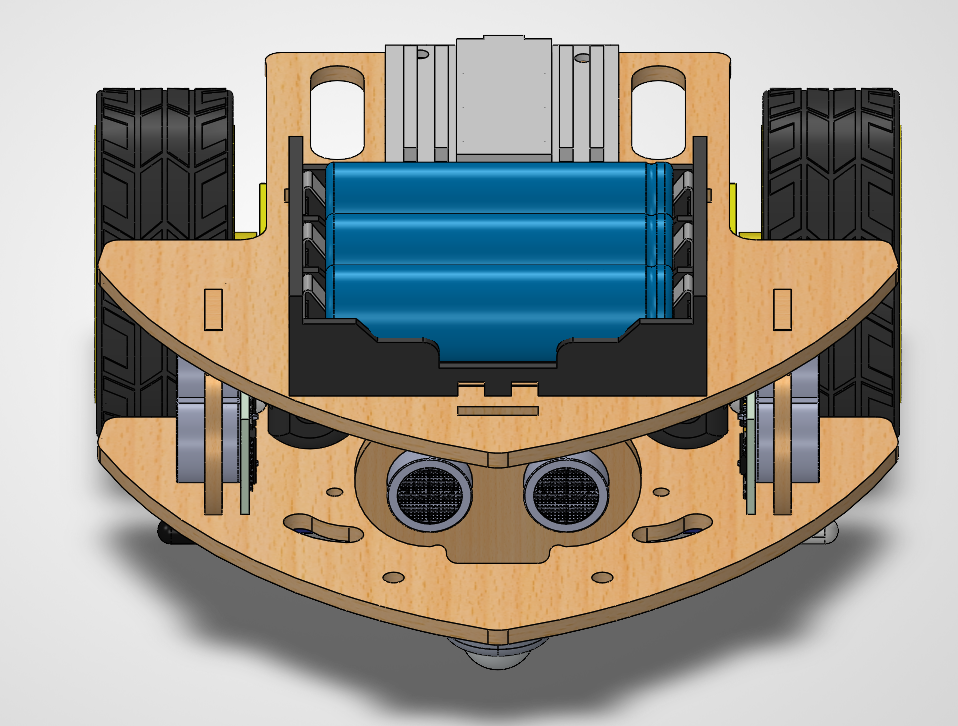
\includegraphics[width=0.7\columnwidth]{cad_1}\\[0.6em]
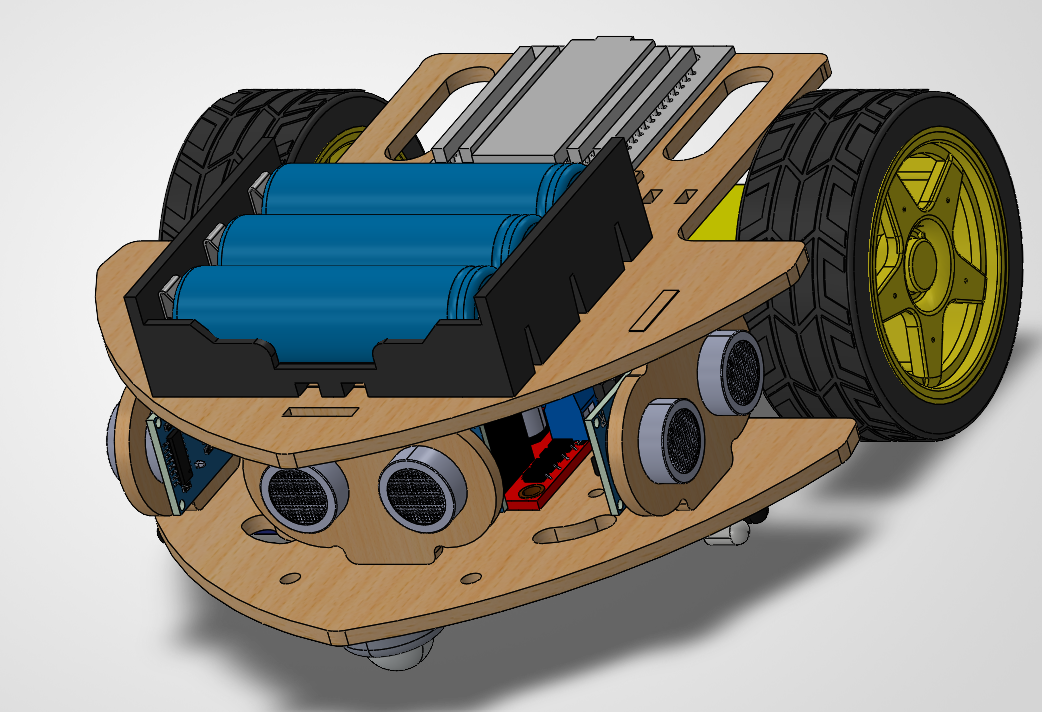
\includegraphics[width=0.7\columnwidth]{cad_2}
\caption{Modelo CAD del chasis del robot móvil: dos vistas del diseño.}
\label{fig:cad}
\end{figure}

No se presentan planos dimensionales definitivos porque las dimensiones del chasis y la separación entre las ruedas todavía están por confirmar.

\begin{table*}[t]
\centering
\caption{Componentes principales seleccionados}
\label{tab:componentes}
\scriptsize
\begin{tabular}{p{0.22\textwidth} p{0.27\textwidth} p{0.43\textwidth}}
\toprule
\textbf{Componente} & \textbf{Función} & \textbf{Por qué se eligió} \\
\midrule
ESP32 & Control y comunicación & Microcontrolador central: ejecuta el firmware, maneja sensores y motores y da conectividad inalámbrica. \\
Motores DC con reductora TT, 6 V, 110 rpm, relación 1:90 & Tracción diferencial & Permiten controlar por separado cada rueda. Cada motor trae un encoder de una salida; su resolución real debe medirse. \\
TB6612FNG & Etapa de potencia & Controla el sentido de giro y la potencia (PWM) de los motores DC. \\
GY-271 con QMC5883L & Medición de orientación & Da mediciones del campo magnético para estimar el rumbo. Necesita calibración y revisión de interferencias. \\
TCS34725 & Detección de color & Entrega lecturas RGB y de intensidad para clasificar colores. \\
HC-SR04 & Detección de obstáculos & Estima distancias por ultrasonido. Su salida ECHO necesita adaptación de nivel. \\
Batería de ion-litio 3S con BMS & Alimentación principal & Da la energía del sistema. Debe usarse con protecciones y convertidores DC-DC. \\
Convertidor reductor a 6 V & Alimentación de motores & Adapta la tensión de la batería al nivel previsto para los motores. \\
Convertidor reductor a 5 V & Alimentación de lógica y periféricos & Da una línea regulada para los módulos que la necesiten; cada uno se alimenta según su hoja de datos. \\
Chasis de acrílico de fabricación propia & Soporte mecánico & Permite ubicar motores, ruedas, sensores y batería según el diseño del proyecto. \\
Pulsador de emergencia & Seguridad & Se propone para detener el sistema y pasar a un estado seguro. Su montaje físico está pendiente. \\
\bottomrule
\end{tabular}
\end{table*}

\subsection{Presupuesto}

Según el presupuesto registrado, el costo total estimado es de \$304\,562 COP y el valor de los elementos que hay que comprar es de \$219\,562 COP. Estos valores son los totales usados para planear y no una cotización verificada en tiempo real.

El desglose por componente está en el archivo \texttt{hardware/BOM.xlsx}. En la versión final se recomienda añadir una tabla con cantidad, precio unitario, subtotal y si el elemento se compra o ya se tiene, usando directamente los datos de ese archivo.

%%%%%%%%%%%%%%%%%%%%%%%%%%%%%%%%%%%%%%%%%%%%%%%%%%%%%%%%%%
%%%%%%%%%%%%%%%%%%%% DISEÑO MECÁNICO %%%%%%%%%%%%%%%%%%%%%%
%%%%%%%%%%%%%%%%%%%%%%%%%%%%%%%%%%%%%%%%%%%%%%%%%%%%%%%%%%

\section{Diseño mecánico}

\subsection{Configuración de la plataforma}

El robot usa una configuración diferencial con dos ruedas motrices independientes y una rueda de apoyo. Esta distribución permite avanzar y retroceder, y girar cambiando la velocidad de cada rueda.

Las ruedas son de $6{,}5~\mathrm{cm}$ de diámetro. Los motores DC con reductora TT se especificaron para $110~\mathrm{rpm}$ y una relación de reducción de $1:90$. Cada motor trae un encoder de una salida, cuyo número real de pulsos por revolución todavía hay que medir.

El chasis se fabricará en acrílico. El modelo CAD está en una etapa inicial, así que aún faltan por definir y documentar las dimensiones definitivas, la separación entre ruedas, la ubicación de los sensores, los soportes de los motores y el espacio para la batería y los convertidores.

\subsection{Consideraciones de diseño}

La distribución mecánica debe cumplir estas condiciones:

\begin{itemize}
    \item Mantener alineados los ejes de las ruedas motrices para reducir desviaciones.
    \item Ubicar el centro de masa para que las ruedas motrices tengan buen contacto con el suelo.
    \item Poner el sensor ultrasónico con visión despejada hacia adelante.
    \item Orientar el sensor de color hacia la superficie y controlar su distancia.
    \item Alejar, en lo posible, el magnetómetro de los motores, los cables de corriente y las piezas metálicas.
    \item Dejar acceso a los conectores, al pulsador de emergencia y a los puntos de mantenimiento.
\end{itemize}

%%%%%%%%%%%%%%%%%%%%%%%%%%%%%%%%%%%%%%%%%%%%%%%%%%%%%%%%%%
%%%%%%%%%%%%%%%%%%%% DISEÑO ELECTRÓNICO %%%%%%%%%%%%%%%%%%%
%%%%%%%%%%%%%%%%%%%%%%%%%%%%%%%%%%%%%%%%%%%%%%%%%%%%%%%%%%

\section{Diseño electrónico}

\subsection{Arquitectura de alimentación}

La alimentación prevista usa una batería de ion-litio de tres celdas en serie con un sistema de gestión (BMS). De la batería salen líneas reguladas para motores y lógica mediante convertidores reductores.

La línea de motores se plantea a $6~\mathrm{V}$ y la de lógica a $5~\mathrm{V}$, según la configuración del proyecto. La tensión que necesita cada módulo debe comprobarse con su hoja de datos antes de montarlo. No hay que suponer que todos los sensores toleran $5~\mathrm{V}$ en sus pines de señal.

Las tierras de los módulos deben compartir una referencia común, cuidando la distribución de corriente para que el paso de corriente por los motores no meta ruido en las señales de los sensores.

El esquema eléctrico definitivo está pendiente y se elaborará antes del montaje físico. Por eso no se incluye todavía un circuito como si ya estuviera implementado.

\subsection{Controlador de motores}

El TB6612FNG se eligió para controlar el sentido de giro y la señal PWM de los motores. Las señales de dirección fijan el sentido y el PWM ajusta la potencia media aplicada.

El pin STBY se conecta a GPIO18 según la asignación preliminar. Debe usarse en nivel bajo para dejar el controlador deshabilitado durante el estado seguro, comprobando que el cableado y el firmware lo cumplan.

Los valores de frecuencia PWM, resolución y límites de velocidad deben definirse en el firmware y probarse con los motores reales. No se presentan velocidades medidas, corrientes de operación ni curvas de respuesta porque esas pruebas físicas aún faltan.

\subsection{Adaptación de señal del sensor ultrasónico}

El pin ECHO del HC-SR04 puede llegar a un nivel mayor del que admite una entrada del ESP32. Por eso se propone un divisor resistivo con una resistencia de $1~\mathrm{k}\Omega$ en serie y una de $2~\mathrm{k}\Omega$ hacia tierra.

La tensión ideal en la salida del divisor es:

\begin{equation}
V_{\mathrm{GPIO}} =
V_{\mathrm{ECHO}}\frac{R_2}{R_1+R_2}
\label{eq:divisor}
\end{equation}

Con $R_1=1~\mathrm{k}\Omega$ y $R_2=2~\mathrm{k}\Omega$, para un nivel ECHO de $5~\mathrm{V}$ se obtiene:

\begin{equation}
V_{\mathrm{GPIO}} =
5\frac{2}{1+2}
\approx 3{,}33~\mathrm{V}
\label{eq:divisor_calculo}
\end{equation}

Este valor es una aproximación ideal. Antes de conectarlo al microcontrolador hay que verificar las tensiones reales, las tolerancias de las resistencias y las condiciones del montaje.

%%%%%%%%%%%%%%%%%%%%%%%%%%%%%%%%%%%%%%%%%%%%%%%%%%%%%%%%%%
%%%%%%%%%%%%%%%%%%%% PINOUT %%%%%%%%%%%%%%%%%%%%%%%%%%%%%%%
%%%%%%%%%%%%%%%%%%%%%%%%%%%%%%%%%%%%%%%%%%%%%%%%%%%%%%%%%%

\section{Asignación preliminar de pines}

La Tabla~\ref{tab:pinout} resume la asignación de pines definida para el firmware. Debe mantenerse igual en los módulos de software, el esquema eléctrico y el montaje físico.

\begin{table*}[t]
\centering
\caption{Asignación preliminar de pines del ESP32}
\label{tab:pinout}
\scriptsize
\begin{tabular}{p{0.24\textwidth} p{0.18\textwidth} p{0.47\textwidth}}
\toprule
\textbf{Módulo o señal} & \textbf{GPIO} & \textbf{Función} \\
\midrule
I2C SDA & GPIO8 & Línea de datos del bus I2C. \\
I2C SCL & GPIO9 & Línea de reloj del bus I2C. \\
HC-SR04 TRIG & GPIO10 & Genera el pulso de disparo ultrasónico. \\
HC-SR04 ECHO & GPIO11 & Entrada del tiempo de retorno, con divisor resistivo. \\
Motor izquierdo IN1 & GPIO4 & Control de dirección del motor izquierdo. \\
Motor izquierdo IN2 & GPIO5 & Control de dirección del motor izquierdo. \\
Motor izquierdo PWM & GPIO6 & Señal PWM del motor izquierdo. \\
Motor derecho IN1 & GPIO7 & Control de dirección del motor derecho. \\
Motor derecho IN2 & GPIO15 & Control de dirección del motor derecho. \\
Motor derecho PWM & GPIO16 & Señal PWM del motor derecho. \\
TB6612FNG STBY & GPIO18 & Habilitación del controlador de motores. \\
Encoder izquierdo A & GPIO12 & Entrada de pulsos del encoder izquierdo. \\
Encoder derecho A & GPIO13 & Entrada de pulsos del encoder derecho. \\
Encoder izquierdo B & GPIO14 & Entrada reservada según la asignación de referencia. \\
Encoder derecho B & GPIO21 & Entrada reservada según la asignación de referencia. \\
Parada de emergencia & GPIO47 & Entrada propuesta para el pulsador de emergencia. \\
\bottomrule
\end{tabular}
\end{table*}

Los nombres de los encoders deben confirmarse con el cableado real. Los motores se describieron con encoder de una salida; por eso los pines adicionales no deben tomarse como canales físicos disponibles hasta verificar el componente comprado. Medir los pulsos por revolución y dejar listas las entradas de encoder quedan pendientes.

\subsection{Sensores conectados por I2C}

Los módulos QMC5883L y TCS34725 comparten el bus I2C previsto. Las direcciones reportadas son $0x0D$ para el QMC5883L y $0x29$ para el TCS34725. Estas direcciones deben confirmarse con una detección del bus en el montaje real.

El bus I2C se prevé a $100~\mathrm{kHz}$. La elección de resistencias pull-up, niveles lógicos y alimentación debe hacerse según las especificaciones de las placas de sensor concretas.

%%%%%%%%%%%%%%%%%%%%%%%%%%%%%%%%%%%%%%%%%%%%%%%%%%%%%%%%%%
%%%%%%%%%%%%%%%%%%%% FIRMWARE %%%%%%%%%%%%%%%%%%%%%%%%%%%%%
%%%%%%%%%%%%%%%%%%%%%%%%%%%%%%%%%%%%%%%%%%%%%%%%%%%%%%%%%%

\section{Desarrollo del firmware}

\subsection{Entorno de desarrollo}

El firmware se desarrolla en C++ con el framework Arduino para ESP32 y la herramienta \texttt{arduino-cli}. La placa objetivo es un ESP32 y la configuración de compilación reportada es:

\begin{lstlisting}[basicstyle=\ttfamily\scriptsize,breaklines=true]
esp32:esp32:esp32s3:PSRAM=opi
\end{lstlisting}

La versión exacta del núcleo del ESP32 debe quedar registrada para poder compilar de forma repetible. La estructura por módulos busca mantener separados los parámetros de hardware, los controladores, la lógica de navegación y la comunicación.

\subsection{Organización por módulos}

La estructura prevista del firmware se organiza en estos módulos:

\begin{itemize}
    \item \texttt{Config}: pines, direcciones de sensores y parámetros de configuración.
    \item \texttt{Diagnostics}: comprobaciones de arranque y diagnóstico.
    \item \texttt{MotorDriver}: señales de dirección y PWM de los motores.
    \item \texttt{Geometry}: cálculos geométricos y parámetros de la plataforma.
    \item \texttt{Compass}: lectura y procesamiento de la brújula.
    \item \texttt{ColorSensor}: lectura y clasificación de color.
    \item \texttt{ObstacleSensor}: lectura de distancia del sensor ultrasónico.
    \item \texttt{Encoder}: conteo de pulsos disponibles.
    \item \texttt{Protocol}: valida los mensajes recibidos y arma las respuestas.
    \item \texttt{Wireless}: comunicación inalámbrica.
    \item \texttt{Telemetry}: organiza las variables que se envían a la aplicación.
    \item \texttt{ControlManual}: interpreta las órdenes de movimiento manual.
    \item \texttt{HeadingControl}: calcula el error de orientación y prepara la corrección de rumbo.
    \item \texttt{NavigationFSM}: cambios de la navegación autónoma.
    \item \texttt{FSMGlobal}: coordina los modos globales del robot.
    \item \texttt{Safety}: parada de emergencia y estado seguro.
\end{itemize}

Que un módulo exista en la arquitectura no significa que ya esté terminado en el hardware. En particular, la comunicación Wi-Fi del firmware, el control completo de orientación, la navegación autónoma integrada y las pruebas de motores necesitan más trabajo.

\subsection{Estado seguro}

El sistema debe arrancar con los motores deshabilitados hasta terminar las comprobaciones iniciales. Ante una parada de emergencia, una pérdida de comunicación, una lectura inválida crítica o un fallo de control, el firmware debe llevar el sistema a un estado seguro.

El pin STBY del controlador de motores está en GPIO18 y se propone mantenerlo en nivel bajo durante el estado seguro. Esto debe acompañarse de una estrategia de firmware que detenga los comandos activos y no reactive los motores hasta cumplir las condiciones de recuperación.

El comportamiento seguro es un requisito de diseño, no algo ya probado en esta entrega.

%%%%%%%%%%%%%%%%%%%%%%%%%%%%%%%%%%%%%%%%%%%%%%%%%%%%%%%%%%
%%%%%%%%%%%%%%%%%%%% COMUNICACIÓN %%%%%%%%%%%%%%%%%%%%%%%%%
%%%%%%%%%%%%%%%%%%%%%%%%%%%%%%%%%%%%%%%%%%%%%%%%%%%%%%%%%%

\section{Comunicación inalámbrica y aplicación}

\subsection{Aplicación de supervisión}

La aplicación de supervisión está hecha a nivel de software y busca permitir el control manual, el cambio de modo, la visualización de variables y la interacción con JARVIS. Falta probarla con el ESP32 físico.

El transporte elegido es WebSocket sobre Wi-Fi. El firmware deberá aceptar conexiones, validar los mensajes, ejecutar los comandos permitidos y devolver las respuestas y la telemetría.

El repositorio del proyecto está en:

\begin{center}
\url{https://github.com/kevinparra943/robot-movil-esp32s3}
\end{center}

\subsection{Formato de mensajes}

El protocolo usa mensajes JSON con los campos comunes de la Tabla~\ref{tab:campos}. La marca de tiempo sirve para ordenar o interpretar eventos según la implementación de cada lado.

\begin{table}[H]
\centering
\caption{Campos comunes del protocolo}
\label{tab:campos}
\scriptsize
\begin{tabular}{p{0.18\columnwidth} p{0.68\columnwidth}}
\toprule
\textbf{Campo} & \textbf{Descripción} \\
\midrule
\texttt{t} & Tipo de mensaje o comando. \\
\texttt{v} & Versión del protocolo; en esta propuesta se usa la versión 1. \\
\texttt{ts} & Marca de tiempo del mensaje. \\
\bottomrule
\end{tabular}
\end{table}

\subsection{Mensajes previstos}

La Tabla~\ref{tab:mensajes} resume los tipos de mensaje previstos entre la aplicación y el robot.

\begin{table*}[t]
\centering
\caption{Mensajes principales del protocolo WebSocket}
\label{tab:mensajes}
\scriptsize
\begin{tabular}{p{0.17\textwidth} p{0.22\textwidth} p{0.51\textwidth}}
\toprule
\textbf{Mensaje} & \textbf{Dirección} & \textbf{Función prevista} \\
\midrule
\texttt{hello} & Aplicación $\rightarrow$ robot & Iniciar el intercambio y comunicar la versión. \\
\texttt{hello\_ack} & Robot $\rightarrow$ aplicación & Confirmar la recepción del mensaje inicial. \\
\texttt{ping} & Aplicación $\rightarrow$ robot & Pedir una respuesta para comprobar el canal. \\
\texttt{pong} & Robot $\rightarrow$ aplicación & Responder a la comprobación. \\
\texttt{mode} & Aplicación $\rightarrow$ robot & Pedir un modo de operación. \\
\texttt{drive} & Aplicación $\rightarrow$ robot & Enviar una orden de movimiento con caducidad. \\
\texttt{heading} & Aplicación $\rightarrow$ robot & Definir una orientación deseada. \\
\texttt{calib} & Aplicación $\rightarrow$ robot & Pedir una calibración permitida. \\
\texttt{estop} & Aplicación $\rightarrow$ robot & Pedir una parada de emergencia. \\
\texttt{status} & Ambas direcciones & Consultar o informar el estado general. \\
\texttt{telemetry} & Robot $\rightarrow$ aplicación & Enviar las variables de sensores y control. \\
\texttt{ack} & Robot $\rightarrow$ aplicación & Confirmar que un mensaje se recibió y procesó. \\
\texttt{error} & Robot $\rightarrow$ aplicación & Avisar de un formato incorrecto o una falla. \\
\texttt{event} & Robot $\rightarrow$ aplicación & Avisar de un evento de funcionamiento. \\
\bottomrule
\end{tabular}
\end{table*}

\subsection{Validación de mensajes y seguridad temporal}

Los mensajes se validan antes de ejecutar una acción. Algunos errores contemplados son:

\begin{itemize}
    \item \texttt{BAD\_FORMAT}: el mensaje está mal formado.
    \item \texttt{UNKNOWN\_CMD}: el comando no se reconoce.
    \item \texttt{UNSUPPORTED}: la operación no está soportada.
    \item \texttt{SAFETY}: el comando se rechaza por seguridad.
    \item \texttt{I2C\_ERROR}: falla la comunicación con un dispositivo I2C.
    \item \texttt{SENSOR\_INVALID}: la lectura es inválida o no está disponible.
    \item \texttt{VERSION\_MISMATCH}: la versión del protocolo no coincide.
\end{itemize}

Para los comandos de movimiento se usa un tiempo de caducidad de $500~\mathrm{ms}$. Si no llega una renovación válida en ese tiempo, el robot debe detenerse y pasar al estado seguro correspondiente. La efectividad de este mecanismo debe probarse con el firmware en el hardware real.

%%%%%%%%%%%%%%%%%%%%%%%%%%%%%%%%%%%%%%%%%%%%%%%%%%%%%%%%%%
%%%%%%%%%%%%%%%%%%%% CONTROL AUTÓNOMO %%%%%%%%%%%%%%%%%%%%%
%%%%%%%%%%%%%%%%%%%%%%%%%%%%%%%%%%%%%%%%%%%%%%%%%%%%%%%%%%

\section{Control manual y navegación autónoma}

\subsection{Control manual}

El control manual permite al usuario pedir movimientos desde la aplicación. Las órdenes se envían con mensajes del protocolo y el firmware comprueba que el modo activo permita el movimiento solicitado.

La velocidad de cada rueda debe limitarse a los valores definidos para el controlador. Cuando llega una orden de parada o vence el comando, las referencias de movimiento deben ponerse en cero.

La aplicación está hecha en software, pero el control manual no se considera validado hasta probar el movimiento físico, el sentido de giro de los motores y la respuesta ante una pérdida de comunicación.

\subsection{Control por voz}

La arquitectura contempla interpretar comandos de voz o texto y convertirlos en acciones reconocidas por el robot. El software de interpretación puede asociar expresiones parecidas con comandos de movimiento o cambio de modo.

La ejecución final debe pasar por el mismo mecanismo de validación y seguridad del control manual. Una orden reconocida por el software no debe mover los motores si el sistema está en estado seguro, en error o en un modo incompatible.

\subsection{Control de orientación}

El control de orientación compara el rumbo actual con el ángulo deseado. El error se calcula con la Ec.~\ref{eq:error_angular}. Con su signo y magnitud, el controlador decide hacia dónde girar y cómo ajustar la velocidad de las ruedas.

La estrategia final debe tener en cuenta el ruido del magnetómetro, el retardo de lectura, la inercia y las perturbaciones magnéticas. La calibración de la brújula y las pruebas de seguimiento de ángulos están pendientes.

\subsection{Evasión de obstáculos}

La evasión debe combinar las mediciones del HC-SR04 con la lógica de navegación. Cuando la distancia cumple la condición de obstáculo, el sistema debe detenerse o reducir el avance, girar y luego decidir si puede continuar.

La distancia de detección, el ángulo de evasión, el tiempo de giro y la condición para retomar el movimiento deben definirse experimentalmente. No se le atribuye al prototipo un número de obstáculos superados hasta hacer y documentar esas pruebas.

\subsection{Detección de seis colores}

La clasificación prevista cubre los colores negro, blanco, rojo, amarillo, verde y azul. Para que sea estable hay que registrar lecturas de referencia con una iluminación parecida a la del lugar de uso.

La calibración debe tener en cuenta la distancia entre el sensor y la superficie, el brillo del material y la luz del ambiente. Los umbrales deben guardarse como parámetros ajustables y probarse con muestras distintas a las usadas para calibrarlos.

%%%%%%%%%%%%%%%%%%%%%%%%%%%%%%%%%%%%%%%%%%%%%%%%%%%%%%%%%%
%%%%%%%%%%%%%%%%%%%% ASISTENTE JARVIS %%%%%%%%%%%%%%%%%%%%%
%%%%%%%%%%%%%%%%%%%%%%%%%%%%%%%%%%%%%%%%%%%%%%%%%%%%%%%%%%

\section{Asistente JARVIS}

El proyecto incluye un asistente llamado JARVIS, hecho con reglas de software. Su función es explicar la arquitectura del robot, responder preguntas sobre sus módulos e informar datos disponibles en la aplicación.

El asistente por reglas asocia palabras clave o intenciones con respuestas ya definidas. Esto da un comportamiento predecible y reduce la dependencia de servicios externos. Su límite son las reglas que se hayan programado y la información que reciba.

La conexión de JARVIS con telemetría real depende de integrar la aplicación con el ESP32. Mientras esa conexión no esté, no se afirma que el asistente esté mostrando mediciones físicas reales de orientación, distancia, color, velocidad o corriente.

La validación futura debe comprobar que las respuestas distingan entre un dato disponible, una lectura inválida y un dato que aún no se ha medido. El asistente no debe inventar datos cuando no haya una medición.

%%%%%%%%%%%%%%%%%%%%%%%%%%%%%%%%%%%%%%%%%%%%%%%%%%%%%%%%%%
%%%%%%%%%%%%%%%%%%%% METODOLOGÍA %%%%%%%%%%%%%%%%%%%%%%%%%%
%%%%%%%%%%%%%%%%%%%%%%%%%%%%%%%%%%%%%%%%%%%%%%%%%%%%%%%%%%

\section{Metodología}

El desarrollo se organiza en etapas para separar el diseño, la implementación de software y la integración física.

\subsection{Etapa 1: análisis de requisitos}

Se identificaron las funciones principales del robot: control manual, comandos de voz, orientación, detección de colores, evasión de obstáculos, comunicación inalámbrica y asistente explicativo. También se definieron requisitos de seguridad, modularidad, validación de mensajes y trazabilidad.

\subsection{Etapa 2: selección de componentes}

Se eligieron el ESP32, el controlador TB6612FNG, los motores TT con reductora, el magnetómetro QMC5883L, el sensor TCS34725 y el sensor ultrasónico HC-SR04. Además se definió una asignación preliminar de pines y una arquitectura de alimentación que necesita un esquema eléctrico definitivo.

\subsection{Etapa 3: diseño mecánico}

Se inició el diseño CAD de un chasis de acrílico con tracción diferencial. El modelo está en una etapa inicial. La fabricación y la verificación de medidas deben completarse antes de fijar los parámetros geométricos finales.

\subsection{Etapa 4: desarrollo de software}

Se desarrollaron módulos de firmware y software para los sensores, la estructura del protocolo, la interpretación de comandos y el asistente JARVIS. Se reporta una compilación del firmware de arranque seguro y sensores, además de pruebas de software ejecutadas sin el robot físico.

\subsection{Etapa 5: validación de software}

Se ejecutaron pruebas para comprobar cálculos, validación de mensajes, interpretación de comandos, respuestas del asistente e integración con un robot simulado por WebSocket. Estas pruebas verifican la parte lógica, pero no reemplazan las mediciones eléctricas y mecánicas del prototipo.

\subsection{Etapa 6: integración y validación física pendiente}

La integración futura incluye armar el esquema eléctrico, probar la alimentación, hacer funcionar los motores, calibrar los sensores, conectar el Wi-Fi real y probar la navegación. Los resultados deben quedar registrados con datos, condiciones de prueba y evidencias fotográficas.

%%%%%%%%%%%%%%%%%%%%%%%%%%%%%%%%%%%%%%%%%%%%%%%%%%%%%%%%%%
%%%%%%%%%%%%%%%%%%%% RESULTADOS DE SOFTWARE %%%%%%%%%%%%%%%
%%%%%%%%%%%%%%%%%%%%%%%%%%%%%%%%%%%%%%%%%%%%%%%%%%%%%%%%%%

\section{Resultados de software}

\subsection{Compilación del firmware}

Se reporta una compilación satisfactoria del firmware de arranque seguro y módulos de sensores. La compilación usó el entorno Arduino para ESP32 y la placa ESP32. El tamaño informado fue de aproximadamente $26\%$ de la memoria de programa y $7\%$ de la memoria global reportada por la herramienta.

Estos porcentajes describen el resultado de compilación y no demuestran que todos los módulos funcionen en el dispositivo físico. La comunicación Wi-Fi, la navegación autónoma y la integración completa de sensores y motores siguen pendientes de validación.

\subsection{Pruebas de software reportadas}

Se reportaron siete grupos de pruebas de software, ejecutados en el entorno de desarrollo, con cero fallos. La Tabla~\ref{tab:pruebas} muestra el alcance de cada uno.

\begin{table*}[t]
\centering
\caption{Pruebas de software reportadas}
\label{tab:pruebas}
\scriptsize
\begin{tabular}{p{0.34\textwidth} p{0.58\textwidth}}
\toprule
\textbf{Prueba} & \textbf{Alcance} \\
\midrule
Normalización angular & Comprobar el cálculo de ángulos y el intervalo del error angular. \\
Clasificación de color & Verificar la lógica de clasificación con entradas de software. \\
Conversión de distancia HC-SR04 & Comprobar la conversión de tiempo de eco a distancia. \\
Protocolo versión 1 & Validar el análisis y la estructura de los mensajes. \\
Interpretación de voz/texto & Comprobar la conversión de expresiones en comandos. \\
Asistente JARVIS & Verificar las respuestas basadas en reglas. \\
Integración WebSocket y caducidad & Evaluar el intercambio de mensajes y la expiración temporal en un entorno simulado. \\
\bottomrule
\end{tabular}
\end{table*}

Estos resultados corresponden a pruebas de software del proyecto. No deben interpretarse como siete pruebas físicas del robot. Para que sean reproducibles, conviene guardar en el repositorio los comandos de ejecución, las versiones de las herramientas, las entradas de prueba, las salidas y los registros de cada corrida.

\subsection{Trazabilidad}

La trazabilidad relaciona los requisitos con los módulos y las pruebas que permiten evaluarlos. La Tabla~\ref{tab:trazabilidad} presenta una relación resumida; el detalle está en \texttt{docs/trazabilidad.md}.

\begin{table*}[t]
\centering
\caption{Trazabilidad resumida entre módulos, pruebas y validación física}
\label{tab:trazabilidad}
\scriptsize
\begin{tabular}{p{0.40\textwidth} p{0.26\textwidth} p{0.26\textwidth}}
\toprule
\textbf{Módulos relacionados} & \textbf{Prueba de software} & \textbf{Validación física pendiente} \\
\midrule
Aplicación, Protocol, ControlManual, MotorDriver & Integración de comandos & Movimiento real y sentido de giro \\
Aplicación, intérprete de comandos, Protocol & Interpretación de voz/texto & Comandos ejecutados en el robot \\
FSMGlobal, Safety, ControlManual, NavigationFSM & Pruebas de lógica de estados por completar & Exclusión de modos y estado seguro \\
Compass, HeadingControl, Geometry & Normalización angular & Calibración y seguimiento de rumbo \\
ColorSensor & Clasificación de color & Lecturas reales de los seis colores \\
ObstacleSensor, NavigationFSM & Conversión de distancia & Detección y evasión en el entorno real \\
Protocol, Wireless, Safety & Protocolo y caducidad en WebSocket simulado & Conexión Wi-Fi y pérdida de comunicación \\
Aplicación web, Telemetry & Integración simulada & Conexión con el ESP32 físico \\
JARVIS, Telemetry, aplicación & Respuestas basadas en reglas & Respuestas vinculadas a variables reales \\
\bottomrule
\end{tabular}
\end{table*}

%%%%%%%%%%%%%%%%%%%%%%%%%%%%%%%%%%%%%%%%%%%%%%%%%%%%%%%%%%
%%%%%%%%%%%%%%%%%%%% LIMITACIONES %%%%%%%%%%%%%%%%%%%%%%%%%
%%%%%%%%%%%%%%%%%%%%%%%%%%%%%%%%%%%%%%%%%%%%%%%%%%%%%%%%%%

\section{Limitaciones y actividades pendientes}

El estado actual del proyecto tiene limitaciones que deben tenerse en cuenta al leer los resultados:

\begin{itemize}
    \item El CAD está en una etapa inicial y todavía deben confirmarse las dimensiones del chasis y la separación entre las ruedas.

    \item El esquema eléctrico definitivo está pendiente. Antes de energizar el sistema hay que verificar la alimentación, la compatibilidad de niveles, la distribución de tierra y las protecciones.

    \item La comunicación Wi-Fi del firmware está pendiente de integración y validación con el ESP32 físico.

    \item La aplicación está hecha, pero no se ha probado con el microcontrolador físico.

    \item JARVIS funciona con reglas de software; su conexión con telemetría física real todavía no está demostrada.

    \item El número real de pulsos por revolución de los encoders debe medirse y documentarse.

    \item Las dimensiones mecánicas definitivas y los parámetros geométricos para la navegación todavía deben establecerse.

    \item La calibración de la brújula y del sensor de color debe hacerse con el montaje final.

    \item Los umbrales de detección de obstáculos, el ángulo de evasión y la estrategia para retomar la trayectoria deben determinarse experimentalmente.

    \item Todavía no hay resultados físicos que demuestren el número de obstáculos superados, la identificación estable de colores o la precisión del seguimiento de rumbo.
\end{itemize}

%%%%%%%%%%%%%%%%%%%%%%%%%%%%%%%%%%%%%%%%%%%%%%%%%%%%%%%%%%
%%%%%%%%%%%%%%%%%%%% PLAN DE VALIDACIÓN %%%%%%%%%%%%%%%%%%%
%%%%%%%%%%%%%%%%%%%%%%%%%%%%%%%%%%%%%%%%%%%%%%%%%%%%%%%%%%

\section{Plan de validación del prototipo}

La guía del proyecto define niveles según el número mínimo de obstáculos y colores reconocidos. Como el nivel definitivo aún está por decidir, la Tabla~\ref{tab:niveles} resume los tres niveles sin afirmar que el robot ya cumpla alguno.

\begin{table}[H]
\centering
\caption{Niveles de alcance indicados en la guía}
\label{tab:niveles}
\scriptsize
\begin{tabular}{c c c}
\toprule
\textbf{Nivel} & \textbf{Obstáculos} & \textbf{Colores} \\
\midrule
1 & Al menos 4 & Al menos 3 \\
2 & Al menos 6 & Al menos 4 \\
3 & Al menos 8 & Al menos 6 \\
\bottomrule
\end{tabular}
\end{table}

Para saber qué nivel se alcanza, cada obstáculo y cada color deben probarse en condiciones registradas. Conviene documentar el entorno, la distancia inicial, el tipo de superficie, la iluminación, el número de intentos, los aciertos, los fallos y la evidencia correspondiente.

\subsection{Pruebas físicas propuestas}

\begin{enumerate}[1.]
    \item \textbf{Alimentación:} verificar las tensiones de salida de los convertidores y que estén dentro de lo que admite cada módulo.

    \item \textbf{Motores:} comprobar el sentido de giro, la respuesta al PWM, la parada y el funcionamiento del pin STBY.

    \item \textbf{Comunicación:} conectar la aplicación con el ESP32 por Wi-Fi, intercambiar mensajes y medir los tiempos de respuesta.

    \item \textbf{Seguridad:} comprobar que los motores se detienen al activar la parada de emergencia y al dejar vencer un comando.

    \item \textbf{Brújula:} comparar la orientación reportada con ángulos conocidos y registrar el error.

    \item \textbf{Colores:} probar cada color previsto con varias muestras y registrar la matriz de clasificación.

    \item \textbf{Obstáculos:} comparar la distancia del HC-SR04 con distancias de referencia y probar las maniobras de evasión.

    \item \textbf{Navegación:} comprobar el control de orientación, el giro hacia el ángulo deseado y la recuperación de la trayectoria tras una evasión.

    \item \textbf{JARVIS:} verificar que las respuestas se basen en datos recibidos y que avise cuando una variable no esté disponible.
\end{enumerate}

Los resultados de estas pruebas se agregarán cuando se realicen. Hasta entonces son actividades pendientes y no se presentan valores de precisión, sensibilidad, aciertos ni tiempos de respuesta físicos.

%%%%%%%%%%%%%%%%%%%%%%%%%%%%%%%%%%%%%%%%%%%%%%%%%%%%%%%%%%
%%%%%%%%%%%%%%%%%%%% CONCLUSIONES %%%%%%%%%%%%%%%%%%%%%%%%%
%%%%%%%%%%%%%%%%%%%%%%%%%%%%%%%%%%%%%%%%%%%%%%%%%%%%%%%%%%

\section{Conclusiones}

\begin{itemize}
    \item Se definió una arquitectura por módulos para un robot móvil basado en ESP32, con subsistemas de accionamiento, percepción, control embebido y supervisión inalámbrica.

    \item Se eligieron los componentes principales: ESP32, motores DC con reductora, controlador TB6612FNG, magnetómetro QMC5883L, sensor de color TCS34725 y sensor ultrasónico HC-SR04.

    \item Se definió una asignación preliminar de pines y se identificaron puntos eléctricos importantes, como adaptar el nivel de ECHO del sensor ultrasónico y verificar las tensiones de alimentación de los módulos.

    \item Se planteó una máquina de estados que separa los modos manual y autónomo e incluye estados de seguridad y error. Su comportamiento debe verificarse en la integración física.

    \item Se desarrolló software para el protocolo, la aplicación, la interpretación de comandos y el asistente JARVIS. Se reportaron siete grupos de pruebas de software sin fallos, incluyendo pruebas de integración con un robot simulado por WebSocket.

    \item Los resultados disponibles son de software y compilación. No permiten concluir que la comunicación Wi-Fi con el ESP32, la navegación autónoma, la detección física de seis colores o la evasión de obstáculos ya estén validadas por completo.

    \item Falta completar el diseño CAD, elaborar el esquema eléctrico definitivo, integrar el Wi-Fi en el firmware, medir los encoders y hacer las pruebas físicas necesarias para saber el nivel de alcance realmente logrado.
\end{itemize}

%%%%%%%%%%%%%%%%%%%%%%%%%%%%%%%%%%%%%%%%%%%%%%%%%%%%%%%%%%
%%%%%%%%%%%%%%%%%%%% TRABAJO FUTURO %%%%%%%%%%%%%%%%%%%%%%%
%%%%%%%%%%%%%%%%%%%%%%%%%%%%%%%%%%%%%%%%%%%%%%%%%%%%%%%%%%

\section{Trabajo futuro}

Estas actividades permitirán pasar de la arquitectura y las pruebas de software a la validación del robot completo:

\begin{enumerate}[1.]
    \item Terminar el modelo CAD, fijar las dimensiones definitivas y fabricar el chasis.

    \item Elaborar el esquema eléctrico completo con las protecciones necesarias.

    \item Confirmar el pinout real, verificar las direcciones I2C y medir los pulsos por revolución de los encoders.

    \item Integrar el servidor Wi-Fi/WebSocket en el firmware y verificar el intercambio de mensajes con la aplicación.

    \item Implementar y validar la parada segura, la caducidad de comandos y la recuperación ante errores.

    \item Calibrar la brújula y el sensor de color en el montaje final.

    \item Ajustar el control de orientación y la estrategia de evasión con pruebas repetibles.

    \item Conectar JARVIS con la telemetría real y comprobar que no contradiga los datos disponibles.

    \item Elegir el nivel de alcance y documentar las pruebas de obstáculos y colores que pide la guía.

    \item Incorporar fotografías propias, diagramas eléctricos definitivos, registros de prueba y resultados cuantitativos.
\end{enumerate}

%%%%%%%%%%%%%%%%%%%%%%%%%%%%%%%%%%%%%%%%%%%%%%%%%%%%%%%%%%
%%%%%%%%%%%%%%%%%%%% REPOSITORIO %%%%%%%%%%%%%%%%%%%%%%%%%%
%%%%%%%%%%%%%%%%%%%%%%%%%%%%%%%%%%%%%%%%%%%%%%%%%%%%%%%%%%

\section{Repositorio del proyecto}

El código fuente y los documentos de desarrollo se organizan en un repositorio de GitHub:

\begin{center}
\url{https://github.com/kevinparra943/robot-movil-esp32s3}
\end{center}

%%%%%%%%%%%%%%%%%%%%%%%%%%%%%%%%%%%%%%%%%%%%%%%%%%%%%%%%%%
%%%%%%%%%%%%%%%%%%%% BIBLIOGRAFÍA %%%%%%%%%%%%%%%%%%%%%%%%%
%%%%%%%%%%%%%%%%%%%%%%%%%%%%%%%%%%%%%%%%%%%%%%%%%%%%%%%%%%

\ifCLASSOPTIONcaptionsoff
  \newpage
\fi

\begin{thebibliography}{11}

\bibitem{Espressif}
Espressif Systems, ``ESP32 Series Datasheet,'' documentación técnica del microcontrolador ESP32. Disponible en: \url{https://www.espressif.com/en/support/documents/technical-documents}

\bibitem{ArduinoESP32}
Espressif Systems, ``Arduino-ESP32 Documentation,'' documentación del framework Arduino para ESP32. Disponible en: \url{https://docs.espressif.com/projects/arduino-esp32/en/latest/}

\bibitem{TB6612}
Toshiba Electronic Devices \& Storage Corporation, ``TB6612FNG Dual DC Motor Driver IC,'' hoja de datos del controlador de motores.

\bibitem{QMC5883L}
QST Corporation, ``QMC5883L 3-Axis Magnetic Sensor,'' documentación técnica del magnetómetro. La hoja de datos debe contrastarse con la revisión del módulo utilizado.

\bibitem{TCS34725}
ams OSRAM, ``TCS3472 Color Light-to-Digital Converter,'' hoja de datos del sensor de color. Disponible en: \url{https://ams-osram.com/}

\bibitem{HCSR04}
ElecFreaks, ``HC-SR04 Ultrasonic Ranging Module,'' documentación técnica del módulo ultrasónico. Se debe verificar la revisión del dispositivo utilizado.

\bibitem{WebSocket}
I. Fette y A. Melnikov, ``The WebSocket Protocol,'' RFC 6455, Internet Engineering Task Force, 2011. Disponible en: \url{https://www.rfc-editor.org/rfc/rfc6455}

\bibitem{JSON}
T. Bray, Ed., ``The JavaScript Object Notation (JSON) Data Interchange Format,'' RFC 8259, Internet Engineering Task Force, 2017. Disponible en: \url{https://www.rfc-editor.org/rfc/rfc8259}

\bibitem{MDN}
Mozilla Foundation, ``MDN Web Docs: WebSocket API,'' documentación técnica. Disponible en: \url{https://developer.mozilla.org/docs/Web/API/WebSocket}

\bibitem{Siegwart}
R. Siegwart, I. R. Nourbakhsh y D. Scaramuzza, \emph{Introduction to Autonomous Mobile Robots}, 2a. ed. Cambridge, MA, EUA: MIT Press, 2011.

\bibitem{GitHub}
GitHub, ``Robot móvil ESP32,'' repositorio del proyecto. Disponible en: \url{https://github.com/kevinparra943/robot-movil-esp32s3}

\end{thebibliography}

\end{document}
